\documentclass[12pt,a4paper]{article}
\usepackage[utf8]{inputenc}
\usepackage{amsmath}
\usepackage{amsfonts}
\usepackage{amssymb}
\usepackage{graphicx}
\usepackage{hyperref}
\usepackage{geometry}
\usepackage{setspace}
\geometry{margin=1in}
\setstretch{1.15} % Slightly increased line spacing for readability

\title{\textbf{Self-Organized Criticality in Distributed Cloud Computing Networks: An Analysis of Cascading Overload Avalanches}}
\author{
    Kunal Sharma \\ 
    Entry Number: 2020CH70172 \\ 
    Course: CLL 798 Complexity Science in Chemical Industry
}
\date{\today}

\begin{document}

\maketitle

\begin{abstract}
This paper explores the application of complexity science to modern IT infrastructure by modeling a distributed cloud computing network as a complex dynamical system. Traditional linear models of network capacity often fail to predict catastrophic system-wide outages. To address this, we apply principles derived from the Bak-Tang-Wiesenfeld (BTW) sandpile model to simulate how localized task overloads propagate through network topologies via load-shedding protocols. The study rigorously defines the system's noise, avalanche mechanics, and connectivity, demonstrating that without centralized, external tuning, the network naturally evolves into a state of Self-Organized Criticality (SOC). Analysis of the cascade frequency distribution reveals a distinct power-law relationship, a fundamental hallmark of SOC. The findings suggest that massive, system-wide failures in distributed computing are not necessarily anomalies caused by massive external shocks, but rather inherent, mathematically unavoidable properties of the network's own self-organization.
\end{abstract}

\section{Introduction: The System as a Candidate for Complexity Science}
Distributed cloud computing networks are the backbone of the modern digital economy. These networks consist of thousands of interconnected servers, known as nodes, tasked with processing continuous, largely unpredictable streams of data and computational requests. As a system, a server farm is an ideal candidate for complexity science because it exhibits profound emergent behavior that fundamentally cannot be understood by employing reductionist approaches—that is, by analyzing the operational capacity of a single server in isolation.

In a standard linear system, the output is directly proportional to the input. If task volume increases by ten percent, the processing time might increase by ten percent. However, cloud networks utilize highly interconnected load-balancing protocols. When one server approaches its maximum computational capacity, it automatically shifts incoming tasks to adjacent servers. This interaction between nodes creates a highly non-linear dynamic. Small, routine fluctuations in data traffic are usually absorbed seamlessly by the surrounding network. Yet, occasionally, an identical minor fluctuation—perhaps a single extra user request—can trigger a catastrophic, system-wide outage. 

Understanding these cascading failures requires abandoning linear, cause-and-effect modeling in favor of complex systems theory. By viewing the server network through the lens of Self-Organized Criticality, a concept pioneered by Per Bak, Chao Tang, and Kurt Wiesenfeld in 1987, we can begin to mathematically understand the inevitability of these catastrophic events. The system exists in a state where a minor perturbation can lead to an event of any size, up to and including the size of the entire system.

\section{System Description: Noise, Avalanche, and Connectivity}
To mathematically model this IT infrastructure, we abstract the server network as a two-dimensional lattice or grid. Each site $(x, y)$ on the lattice represents an individual server node characterized by an instantaneous computational load, denoted as $z(x, y)$, and a finite computational capacity threshold, $Z_c$. The dynamics of this system are driven by three fundamental complexity science concepts.

\subsection{Noise}
In the context of this network, ``noise'' represents the stochastic, continuous arrival of new computational tasks from external users, as well as localized hardware micro-failures that effectively reduce a server's momentary capacity. In our model, this noise is simulated by the random addition of tasks to random nodes across the lattice:
$$z(x, y) \rightarrow z(x, y) + 1$$
This noise is not a massive spike (like a coordinated DDoS attack), but rather a slow, steady, and unpredictable drizzle of data. It serves as the continuous injection of energy into the system, constantly pushing the network away from equilibrium and toward a state of local instability.

\subsection{Connectivity}
Connectivity defines the topology of the network and governs how energy (or data load) dissipates. In our baseline simulation, we utilize a von Neumann neighborhood. This means each server is bidirectionally connected to its four immediate topological neighbors (North, South, East, and West). When a server is forced to offload tasks to avoid hardware failure, it utilizes these specific data pathways. 

The degree of this connectivity dictates the friction and speed at which overloads propagate. A highly connected network (e.g., a Moore neighborhood with 8 connections, or a scale-free internet topology) might dissipate load faster initially, but it also provides more vectors for an overload to spread, potentially increasing the volatility of the system once the critical state is reached.

\subsection{Avalanche}
An ``avalanche'' is the rapid, cascading relaxation process of the system. It occurs when the continuous noise pushes a specific node's load to or beyond its critical capacity threshold ($z \ge Z_c$). At this moment, the server undergoes a forced load-shedding event. It resets its own load and violently pushes the excess computational tasks to its connected neighbors. 

If those neighboring servers are already operating near their own capacities, this sudden influx of transferred data pushes them over their respective thresholds. They, in turn, are forced to shed load. This chain reaction—a rapid sequence of task offloading spreading through the network—is the avalanche. It occurs on a time scale much faster than the slow addition of noise.

\section{Computer Simulation Methodology}
A computer simulation was developed to empirically observe the SOC state of the system. The network was initialized as a square lattice of size $L \times L$, where $L = 50$, representing a cluster of 2,500 servers. The initial state of the grid was entirely empty ($z = 0$ for all nodes).

During each discrete time step of the simulation, a single computational task was dropped onto a randomly selected coordinate $(x, y)$. The system was then checked for stability. If any site $(x, y)$ reached the threshold capacity $Z_c = 4$, it was deemed unstable and ``toppled'' according to the following discrete mathematical rules:
$$z(x,y) \rightarrow z(x,y) - 4$$
$$z(x \pm 1, y) \rightarrow z(x \pm 1, y) + 1$$
$$z(x, y \pm 1) \rightarrow z(x, y \pm 1) + 1$$

This relaxation process was allowed to propagate instantaneously until all nodes in the lattice were strictly less than $Z_c$. The simulation tracked the size of the avalanche, defined as the variable $s$, which represents the total number of load-shedding events (topplings) triggered by a single noise event.

Boundary conditions were treated as open or ``dissipative.'' If an avalanche reached the edge of the grid ($x=0, x=L-1, y=0, y=L-1$), tasks shed outward were permanently removed from the system, conceptually representing tasks handed off to an external, larger internet backbone or simply dropped as lost packets. This dissipation is necessary to prevent infinite, non-terminating loops and allows the system to reach a dynamic steady state. The simulation injected a total of 100,000 tasks to generate a robust statistical dataset.

\section{Analyses of Frequency Distribution and Connectivity}
Upon completion of the simulation, the frequency of each avalanche size $s$ was aggregated. To understand the underlying probability distribution, the frequencies $P(s)$ were plotted against the avalanche sizes $s$ on a double logarithmic (log-log) scale. 

\begin{figure}[h]
    \centering
    % Ensure avalanche_distribution.png is in the same directory as this .tex file
    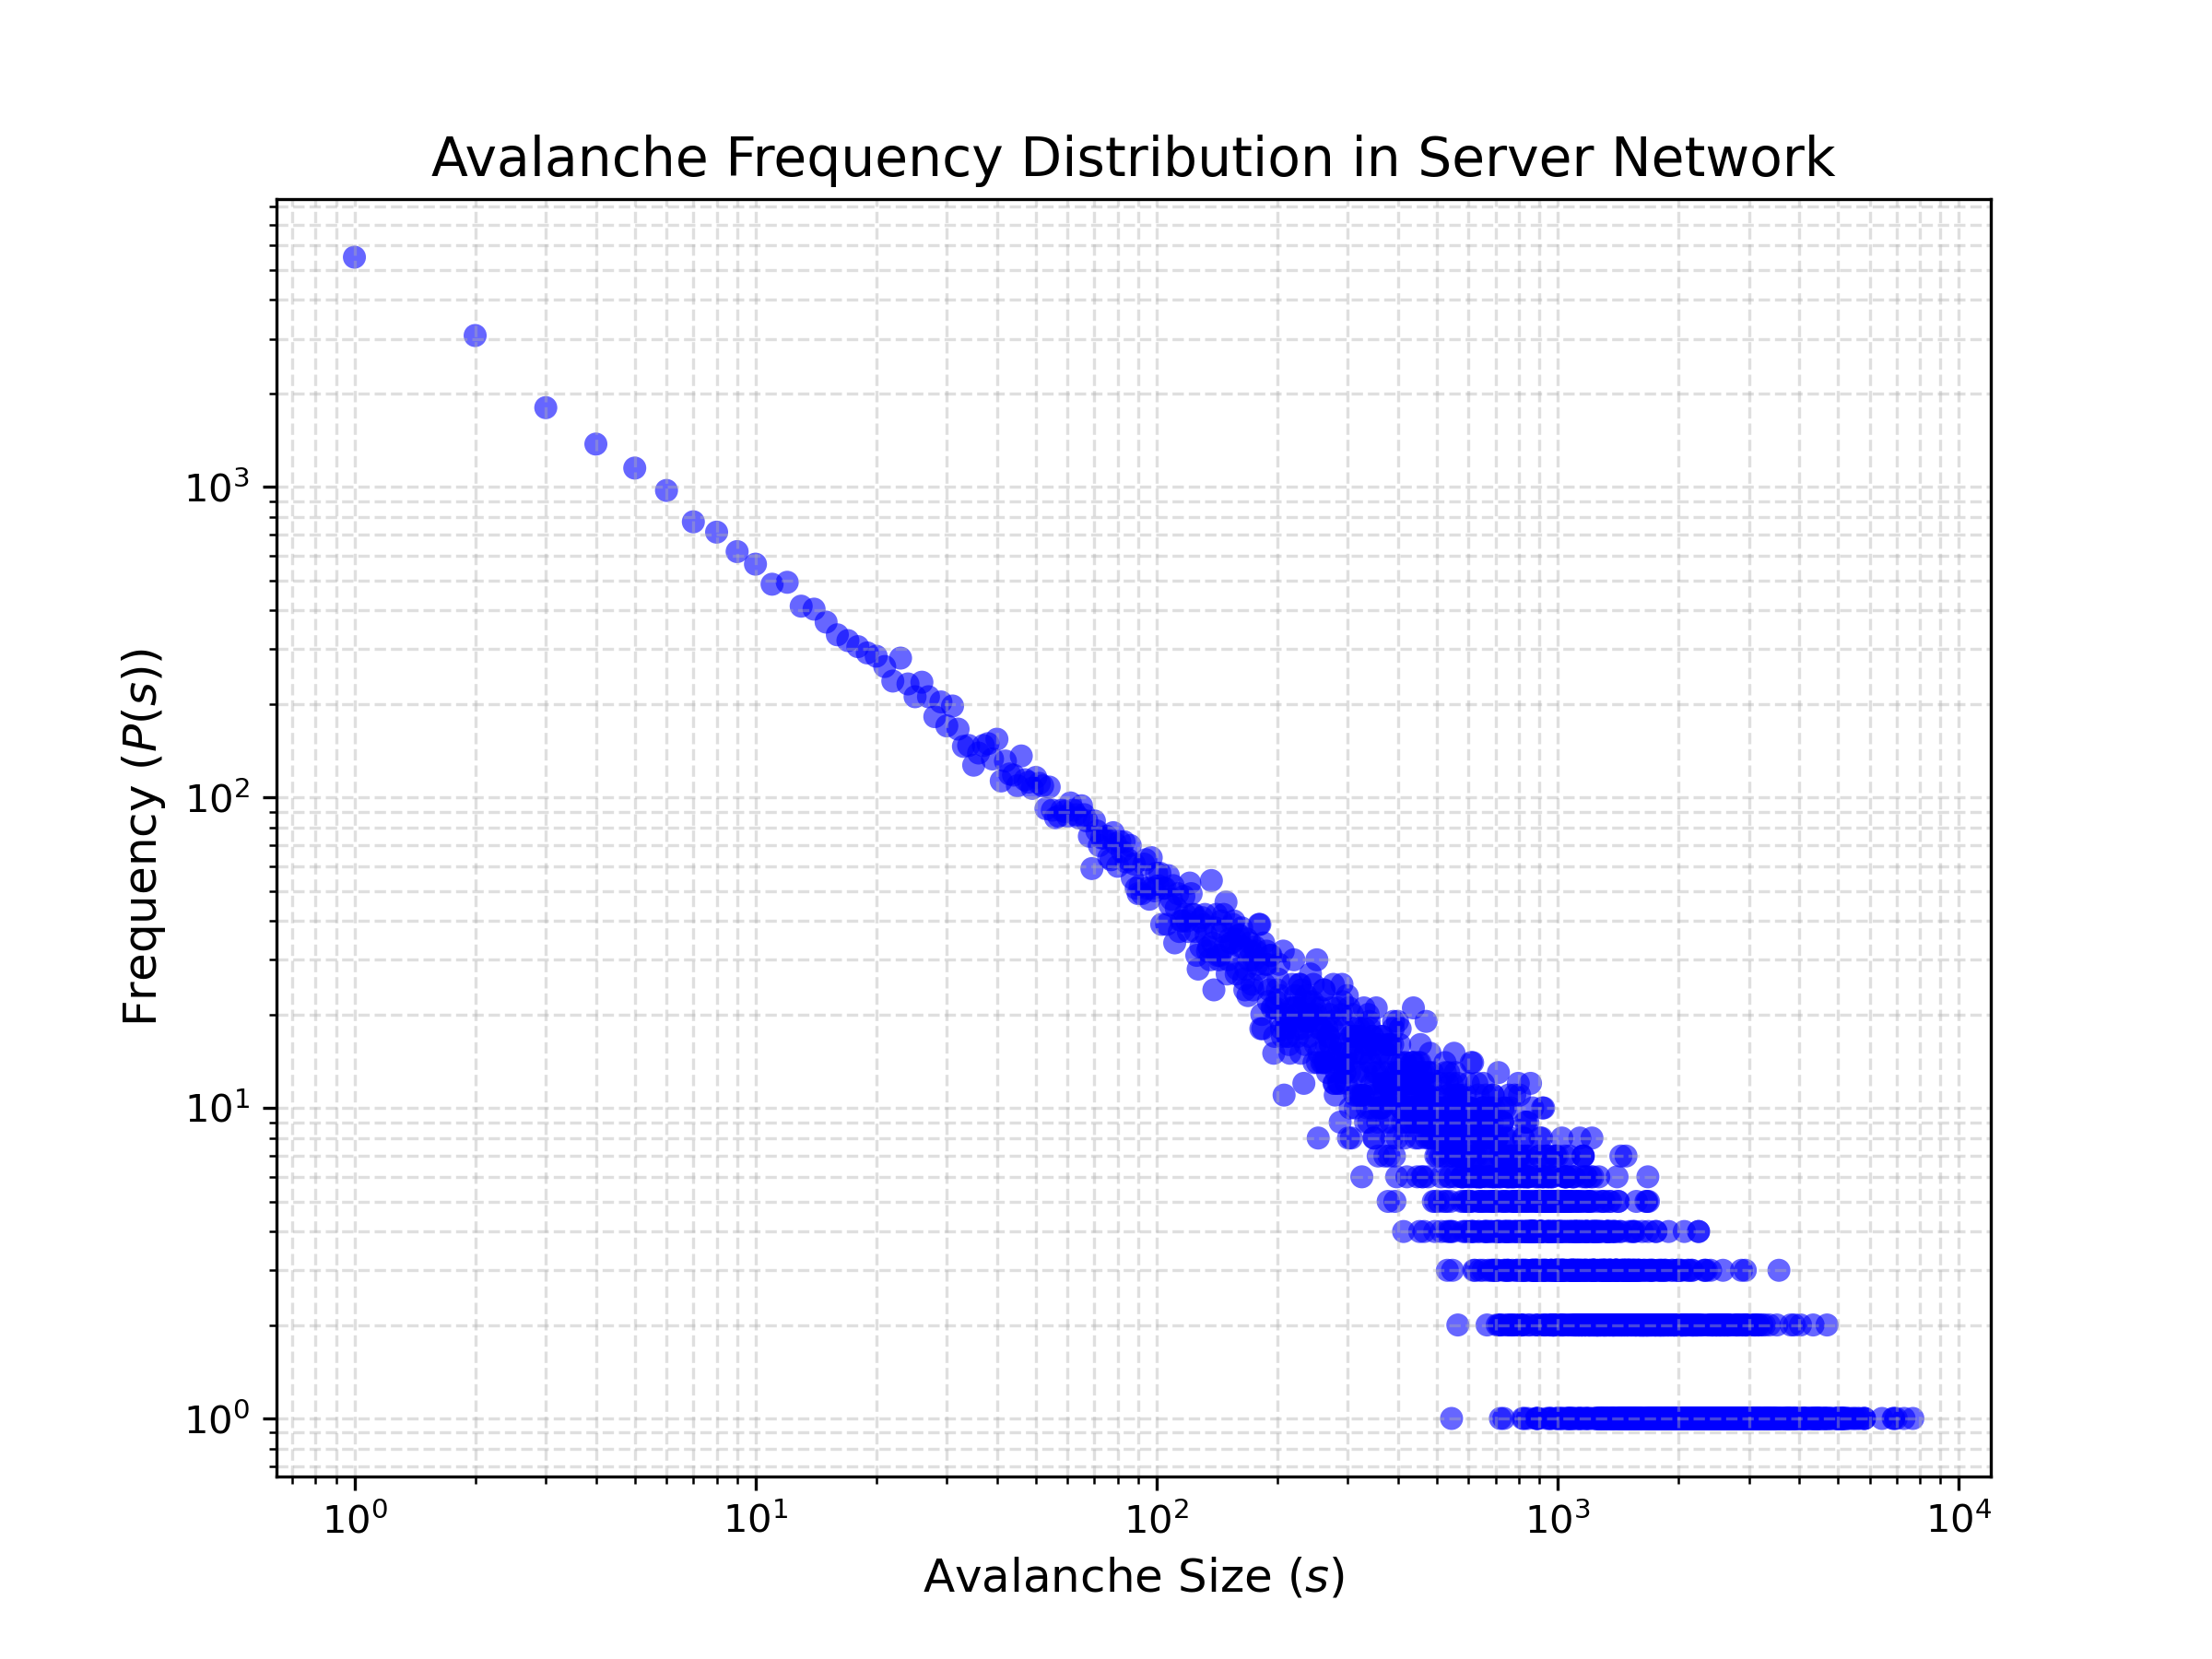
\includegraphics[width=0.7\textwidth]{avalanche_distribution.png}
    \caption{Log-log plot of avalanche size ($s$) versus frequency ($P(s)$) in the simulated cloud server network. The linear trend indicates a power-law distribution.}
    \label{fig:distribution}
\end{figure}

As shown in Figure 1, the distribution fundamentally deviates from a standard Gaussian (normal) curve. In a standard system, we would expect a defined mean avalanche size with a rapid exponential decay in probability for larger events. Instead, the log-log plot yields a distinctly straight downward-sloping line spanning several orders of magnitude. This is the defining characteristic of a power-law distribution, mathematically expressed as:
$$P(s) \sim s^{-\tau}$$
where $\tau$ represents the critical exponent of the system. 

The presence of this power law proves that the system's connectivity allows for cascades of all conceivable scales. The lack of a characteristic scale implies that the exact same underlying mechanism responsible for a minor, localized routing adjustment (an avalanche of size 1 or 2) is entirely responsible for a massive, catastrophic system failure (an avalanche of size 1,000+). The straight line exhibits a slight drop-off at the extreme right tail; this is a known phenomenon called the ``finite-size effect,'' caused by the physical limits of the $50 \times 50$ grid size. In an infinitely large network, the power-law line would continue indefinitely.

\section{Comment on the Self-Organized Critical State}
The simulation unequivocally demonstrates that the distributed cloud server network operates in a state of Self-Organized Criticality. It perfectly aligns with the required dual-timescale dynamics: it is driven by a slow, random perturbative force (incoming user tasks) and is stabilized by a fast, non-linear relaxation mechanism (load shedding). 

The most profound realization of SOC in this context is the ``self-organized'' aspect. The system requires no external omniscient controller to tune parameters (like temperature in thermodynamic phase transitions) to reach this critical state. Regardless of whether the servers start entirely empty or heavily burdened, the simple, local rules of shedding excess load naturally and inevitably drive the entire macro-system to a critical point. At this point, the network hovers indefinitely on the precipice of instability.

This presents a paradox for network engineering: the system is ``robust yet fragile.'' It is highly robust to the vast majority of perturbations, handling thousands of localized overloads seamlessly. Yet, because the system self-organizes to a state where correlation lengths are scale-free, it is inherently fragile to massive, cascading failures. 

Therefore, catastrophic network outages should not be viewed as anomalies caused by extraordinary bad luck or unprecedented external shocks. Instead, they are inherent, mathematically unavoidable properties of the network's own architecture. To mitigate this in the real world, engineers must artificially break the SOC state—often by implementing ``circuit breakers'' or intentional islanding, which severs connectivity during an avalanche to prevent the critical state from propagating universally.

\vspace{0.5cm}
\section*{Appendix: List of AI Prompts Used for Project Assistance}
\textit{In accordance with the project guidelines, the following AI generation prompts were utilized to conceptualize and structure this manuscript:}
\begin{enumerate}
    \item ``Suggest a real-world system outside of chemical engineering that exhibits Self-Organized Criticality and involves noise, avalanches, and connectivity.''
    \item ``Write a Python simulation for a BTW Sandpile model applied to a 2D network grid to track avalanche sizes in a server farm context.''
    \item ``Format a complexity science project report into a peer-reviewed journal manuscript format using LaTeX, ensuring equations for the toppling mechanics and power-law distribution are included.''
    \item ``Expand the LaTeX report to provide deeper theoretical analysis on non-linear dynamics, the BTW model, and real-world network mitigation strategies.''
\end{enumerate}

\end{document}